% !TEX root = ./article.tex

\documentclass{article}

\usepackage{mystyle}
\usepackage{myvars}



%-----------------------------

\begin{document}

	\maketitle % Insert title

	\thispagestyle{fancy} % All pages have headers and footers


%-----------------------------
%	ABSTRACT
%-----------------------------

	\begin{abstract}
		\noindent [TODO ]
	\end{abstract}

%-----------------------------
%	TEXT
%-----------------------------
	\section{Introducción}
	\label{sec:intro}

		\paragraph{}
		[TODO ]


	\section{Redes Bayesianas}
	\label{sec:bayes_network}

		\paragraph{}
		[TODO ]

		\subsection{Estructura Naive Bayes}
		\label{sec:structure_naive}

			\paragraph{}
			[TODO ]


		\subsection{Estructura TAN}
		\label{sec:structure_tan}

			\paragraph{}
			[TODO ]


		\subsection{Estructura K2}
		\label{sec:structure_K2}

			\paragraph{}
			[TODO ]



	\section{Experimentos}
	\label{sec:experiments}

		\paragraph{}
		Tras haber descrito las \emph{Redes Bayesianas} en la sección anterior, a continuación se presentan los resultados obtenidos tras realizar un conjunto de experimentos sobre el conjunto de datos \textbf{Credit}, que se describen en la sección \ref{data_set}. Los tests han consistido en la evaluación del comportamiento de los algoritmos de generación de \emph{Redes Bayesianas} implementadas en \emph{Weka} \cite{tool:weka} variando el tamaño de los conjuntos de entrenamiento.

		\paragraph{}
		La metodología seguida ha sido la siguiente: Para cada conjunto de datos de entrenamiento se ha realizado un experimento de \emph{Validación Cruzada de 10 particiones} a partir del cual se ha almacenado la tasa de error obtenida. Además, se han guardado los modelos generados en cada caso para después probarlos sobre un conjunto de datos independiente del de entrenamiento. Esta tarea se ha repetido con tres los conjuntos de datos de 3 tamaños diferentes sobre los algoritmos de generación de \emph{Redes Bayesianas} descritos en la sección anterior: \emph{Naive Bayes}, \emph{K2} y \emph{TAN}.

		\paragraph{}
		A continuación se describe la naturaleza del conjunto de datos utilizado para los experimentos así como los tamaños de sus particiones.

		\subsection{Conjunto de Datos}
		\label{sec:data_set}

			\paragraph{}
			El conjunto de datos utilizado se denomina \emph{Credit} y se puede acceder a él a través de \url{https://github.com/garciparedes/machine-learning-bayesian-2/tree/master/weka/datasets} \cite{garciparedes:machine-learning-bayesian-2}. Está formado por \textbf{11 atributos} de carácter nominal más la clase de destino formada por \textbf{2 valores}. Dichos atributos presentan un rango de valores reducidos, encontrandose todos ellos entre \textbf{2 y 4 valores distintos}.

			\paragraph{}
			En cuanto a los conjuntos de datos utilizados para los experimentos, todos ellos contienen los mismos atributos así como instancias representativas para todos los valores posibles de los atributos. Tampoco se dan atributos desconocidos. a continuación se describen los tamaños de cada conjunto de datos:

			\begin{itemize}
				\item \textbf{Datos\_Credit\_100}: Está formado por $100$ instancias.
				\item \textbf{Datos\_Credit\_1000}: Está formado por $1000$ instancias.
				\item \textbf{Datos\_Credit\_10000}: Está formado por $10000$ instancias.
				\item \textbf{Test\_Credit\_1000}: Está formado por $1000$ instancias.
			\end{itemize}

			\paragraph{}
			Por último es necesario describir tanto el estimador como los parámetros de configuración utilizados para cada algoritmo. En cuanto al \emph{método de estimación} de probabilidades, se ha escogido el \emph{Estimador de Máxima Verosimilitud con corrección de Laplace} y $m = 0.5$. Dicho estimador se muestra en la ecuación \eqref{eq:naive_bayes_smoothing}, donde $n_c$ representa el número de ejemplos de entrenamiento con la clase $b_j$, $n$ el número de ejemplos de la de entrenamiento con la clase $b_j$ y el atributo $a_i$. El valor $p$ se obtiene mediante $p = Pr(A = a_i | B = b_j)$, es decir, la estimación a priori y $m$ un determinado peso para la estimación a priori.

			\begin{equation}
			\label{eq:naive_bayes_smoothing}
			 Pr'(A = a_i | B = b_j) = \frac{n_c + mp}{n + m}
			\end{equation}

			\paragraph{}
			En cuanto a los algoritmos de clasificación, \emph{Naive Bayes} no tiene más parámetros adicionales. \emph{K2} se ha configurado para que no comience de una red \emph{Naive Bayes} y se ha permitido que cada nodo tenga un número arbitrario de padres. En el caso de \emph{TAN}, se ha seleccionado el método de puntuación de \emph{Máxima Verosimilitud con corrección de Laplace} descrito en la ecuación \eqref{eq:naive_bayes_smoothing} con parámetro $m = 0.5$ al igual que en el caso del método de estimación de probabilidades.

		\paragraph{}
		En la sección \ref{sec:results} se presentan los resultados obtenidos así como una discusión acerca de los mismos.

		\subsection{Resultados}
		\label{sec:results}

			\paragraph{}
			En la figura \ref{fig:bayes_network} se muestra la estructura de las distintas \emph{Redes Bayesianas} generadas por cada algoritmos dependiendo del tamaño del conjunto de datos de entrenamiento. Nótese que estas redes han sido generadas a partir de un experimento de \emph{Validación Cruzada de 10 particiones} sobre conjuntos de datos de \emph{100}, \emph{1000} y \emph{10000} instancias respectivamente.

			\paragraph{}
			En cuanto al algoritmo \emph{Naive Bayes}, la estructura de la red generada es trivial en ambos casos, suponiendo dependencia directa de la clase sobre todos los atributos, por lo que se genera un árbol de profundidad $1$ donde el nodo raiz es la clase y los nodos hoja se corresponden con los $11$ atributos. Nótese que el tamaño del conjunto de datos de entrenamiento no genera variaciones tal y como se muestra en las figuras \ref{fig:naive_100}, \ref{fig:naive_1000} y \ref{fig:naive_10000}.

			\paragraph{}
			Las redes generadas por el algoritmo \emph{K2} presentan una característica diferenciadora respecto del resto. En este caso no todos los atributos tienen como padre al nodo referido a la \emph{clase} (algunos a pesar de no ser la clase de destino no tienen padre). Esto se traduce de manera práctica en que dichos atributos no serán utilizados durante las fases de clasificación de nuevas instancias. La razón es la estrategia de construcción de redes seguida por este algoritmo, que añade una arista tan solo cuando la puntuación obtenida mediante el indicador de verosimilitud se mejora. Las estructuras generadas a partir de cada conjunto de datos de distinto tamaño se muestran en las figuras \ref{fig:k2_100}, \ref{fig:k2_1000} y \ref{fig:k2_10000}.

			\paragraph{}
			[TODO descripción TAN]

			\begin{figure}[h]
				\centering
				\begin{subfigure}{.32\textwidth}
					\centering
					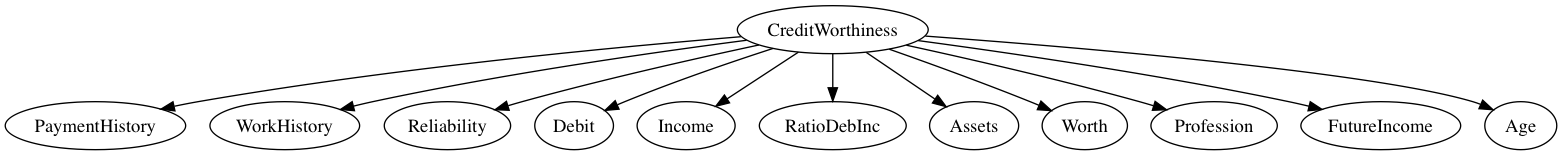
\includegraphics[width=\linewidth]{bayesnet-simple-100}
					\caption{Naive Bayes - 100}
					\label{fig:naive_100}
				\end{subfigure} \
				\begin{subfigure}{.32\textwidth}
					\centering
					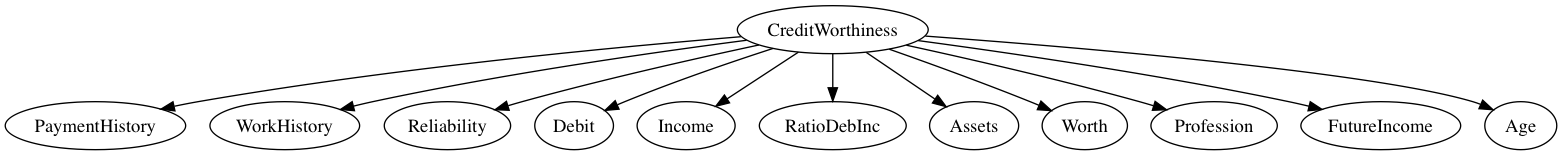
\includegraphics[width=\linewidth]{bayesnet-simple-1000}
					\caption{Naive Bayes - 1000}
					\label{fig:naive_1000}
				\end{subfigure} \
				\begin{subfigure}{.32\textwidth}
					\centering
					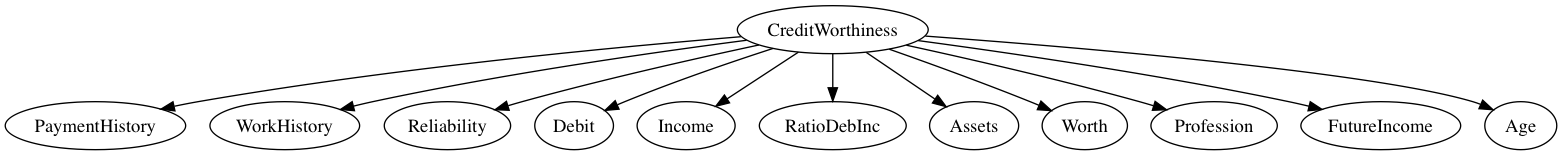
\includegraphics[width=\linewidth]{bayesnet-simple-10000}
					\caption{Naive Bayes - 10000}
					\label{fig:naive_10000}
				\end{subfigure} \\
				\begin{subfigure}{.32\textwidth}
					\centering
					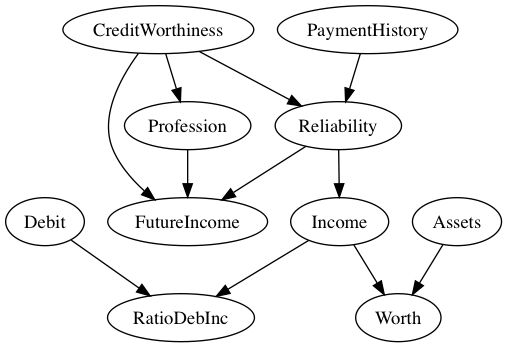
\includegraphics[width=\linewidth]{bayesnet-k2-100}
					\caption{K2 - 100}
					\label{fig:k2_100}
				\end{subfigure} \
				\begin{subfigure}{.32\textwidth}
					\centering
					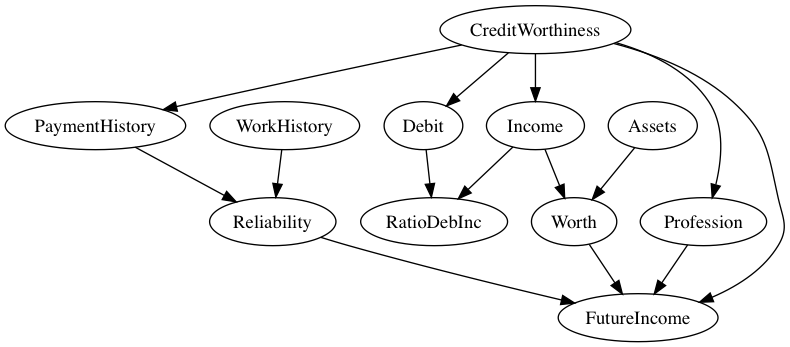
\includegraphics[width=\linewidth]{bayesnet-k2-1000}
					\caption{K2 - 1000}
					\label{fig:k2_1000}
				\end{subfigure} \
				\begin{subfigure}{.32\textwidth}
					\centering
					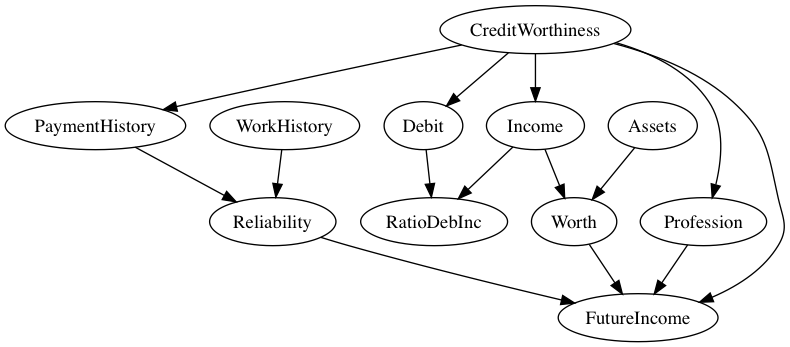
\includegraphics[width=\linewidth]{bayesnet-k2-1000}
					\caption{K2 - 10000}
					\label{fig:k2_10000}
				\end{subfigure} \\
				\begin{subfigure}{.32\textwidth}
					\centering
					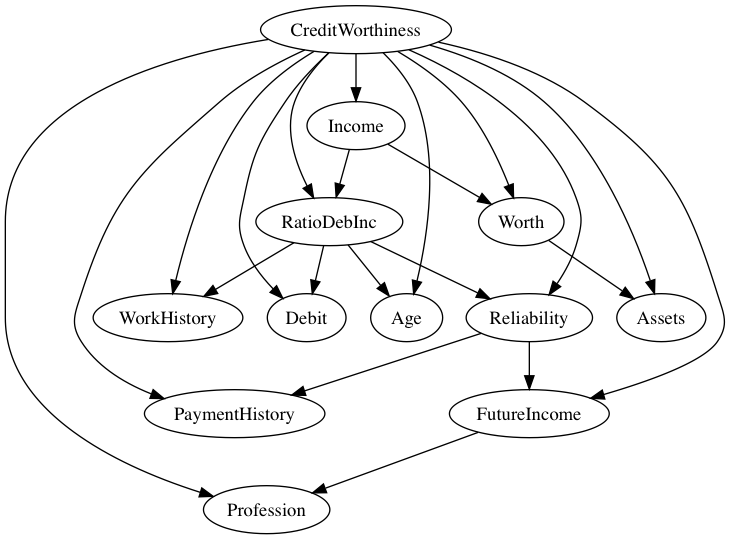
\includegraphics[width=\linewidth]{bayesnet-tan-100}
					\caption{TAN - 100}
					\label{fig:tan_100}
				\end{subfigure} \
				\begin{subfigure}{.32\textwidth}
					\centering
					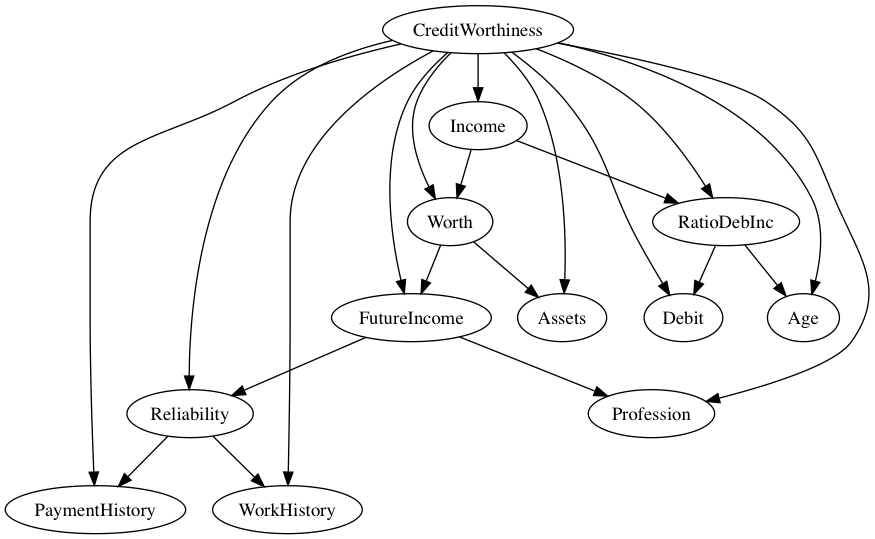
\includegraphics[width=\linewidth]{bayesnet-tan-1000}
					\caption{TAN - 1000}
					\label{fig:tan_1000}
				\end{subfigure} \
				\begin{subfigure}{.32\textwidth}
					\centering
					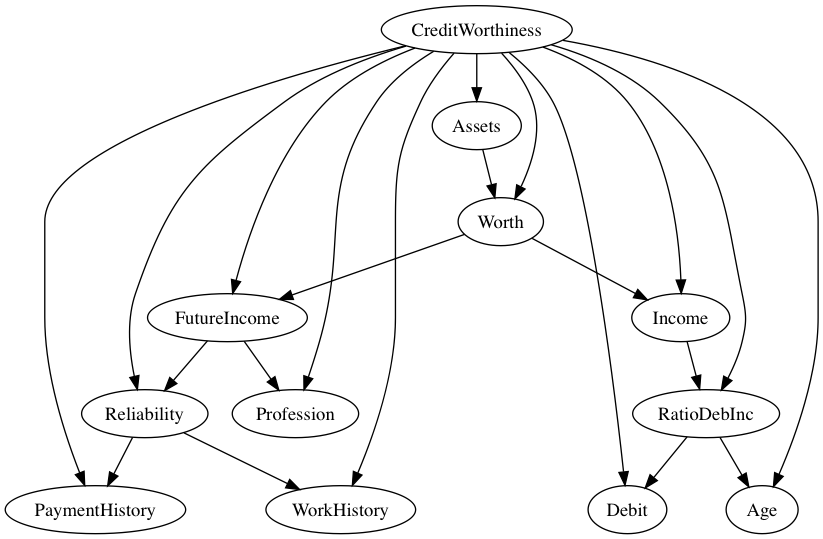
\includegraphics[width=\linewidth]{bayesnet-tan-10000}
					\caption{TAN - 10000}
					\label{fig:tan_10000}
				\end{subfigure}
				\caption{Redes Bayesianas generadas a partir de DatosCredit}
				\label{fig:bayes_network}
			\end{figure}


			\paragraph{}
			[TODO ]

			\begin{table}
			\centering
			\small
			\begin{tabu}{ | c | c | c | c | c | c | c | c | c | c | }
				\hline
				\multicolumn{10}{ | c | }{Clasificación mediante Redes Bayesianas} \\ \hline
				\multirow{3}{*}{Datos}& \multicolumn{9}{ c |}{Tasa de Error} \\ \cline{2-10}
															& \multicolumn{3}{ c |}{Naive Bayes} & \multicolumn{3}{ c |}{K2} & \multicolumn{3}{ c |}{TAN}\\ \cline{2-10}
															& \emph{100} & \emph{1000} & \emph{10000} & \emph{100} & \emph{1000} & \emph{10000} & \emph{100} & \emph{1000} & \emph{10000}\\ \hline
				Entrenamiento		& $36.000\%$	 & $31.700\%$ & $29.690\%$ & $28.000\%$	 & $36.100\%$ & $28.500\%$	& $35.000\%$ & $29.500\%$ & $28.270\%$	\\ \hline
				Datos Test			& $30.000\%$	 & $27.800\%$ & $27.500\%$ & $33.300\%$	 & $30.400\%$ & $25.400\%$	& $33.300\%$ & $24.900\%$ & $25.000\%$	\\
				\hline
			\end{tabu}
			\caption{Tasas de error obtenida a partir de distintas configuraciones de \emph{Redes Bayesianas}}
			\label{table:error_rates}
		\end{table}


%-----------------------------
%	Bibliographic references
%-----------------------------
	\nocite{garciparedes:machine-learning-bayesian-2}
	\nocite{subject:taa}
	\nocite{tool:weka}
  \bibliographystyle{alpha}
  \bibliography{bib/misc}

\end{document}
